\htmlhr
\section{IGJ (immutability) checker\label{igj-checker}}

IGJ is a Java language extension that helps programmers to avoid mutation errors
(unintended side effects).
If the IGJ checker issues no warnings for a given program, then that program
will never change objects that should not be changed.  This guarantee
enables a programmer to detect and prevent mutation-related errors.
(See Section~\ref{checker-guarantees} for caveats to the guarantee.)


\subsection{IGJ and Mutability\label{igj-and-mutability}}

IGJ permits a
programmer to express that a particular object should never be modified via any
reference (object immutability), or that a reference should never be used to
modify its referent (reference immutability). Once a programmer has expressed
these facts, an automatic checker analyzes the code to either locate mutability
bugs or to guarantee that the code contains no such bugs.

\begin{figure}
\begin{center}
\resizebox{!}{3.5cm}{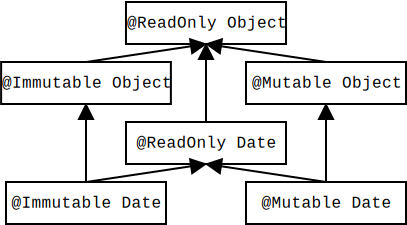
\includegraphics{figures/igj}}
\end{center}
%BEGIN LATEX
\vspace{-1.5\baselineskip}
%END LATEX
\caption{Type hierarchy for three of IGJ's type qualifiers.}
\label{fig:igj-hierarchy}
\end{figure}

To learn the details of the IGJ language and type system, please see the
ESEC/FSE 2007 paper ``Object and reference immutability using Java
generics''~\cite{ZibinPAKE2007}.
The IGJ checker supports Annotation IGJ (Section~\ref{annotation-igj-dialect}),
which is slightly different dialect
of IGJ than that described in the ESEC/FSE paper.


\subsection{IGJ Annotations\label{igj-annotations}}

Each object is either immutable (it can never be modified) or mutable (it
can be modified).  The following qualifiers are part of the IGJ type system.

\begin{description}

\item[\code{@\refclass{igj/quals}{Immutable}}]
  An immutable reference always refers to an immutable object.  Neither the
  reference, nor any aliasing reference, may modify the object.

\item[\code{@\refclass{igj/quals}{Mutable}}]
  A mutable reference refers to a mutable object.  The reference, or some
  aliasing mutable reference, may modify the object.

\item[\code{@\refclass{igj/quals}{ReadOnly}}]
  A readonly reference cannot be used to modify its referent.  The referent
  may be an immutable or a mutable object.  In other words, it is possible
  for the referent to change via an aliasing mutable reference, even though
  the referent cannot be changed via the readonly reference.

\item[\code{@\refclass{igj/quals}{AssignsFields}}]
  is similar to \<@Mutable>, but permits only limited mutation ---
  assignment of fields --- and is intended for use by constructor helper
  methods.

\item[\code{@\refclass{igj/quals}{I}}]
  simulates mutability overloading or the template behavior of generics.
  It can be applied to classes, methods, and parameters.  See
  Section~\ref{igj-templating}.

\end{description}

For additional details, see~\cite{ZibinPAKE2007}.


\subsection{What the IGJ checker checks\label{igj-checks}}

The IGJ checker issues an error whenever mutation happens through a
readonly reference, when fields of a readonly reference which are not
explicitly marked with \code{@\refclass{igj/quals}{Assignable}} are
reassigned, or when a readonly expression is assigned to a mutable
variable.  The checker also emits a warning when casts increase the
mutability access of a reference.

% There is no visitor to reference!
% For a complete description of all checks performed by
% the checker, see the Javadoc for \refclass{igj}{IGJVisitor}.


\subsection{Implicit qualifiers}

As described in Section~\ref{effective-qualifier}, the IGJ checker
adds implicit qualifiers, reducing the number of annotations that must
appear in your code.
% For example, ...

For a complete description of all implicit nullness qualifiers, see the
Javadoc for \refclass{nullness}{NullnessAnnotatedTypeFactory}.

The default annotation (for types that are unannotated and not given an
implicit qualifier) is as follows:
\begin{itemize}
\item
  \code{@Mutable} for almost all references.  This is backward-compatible
  with Java, since Java permits any reference to be mutated.
\item
  \code{@Readonly} for local variables.  This qualifier may be refined by
  flow-sensitive local type refinement (see Section~\ref{type-refinement}).
\item
  \code{@Readonly} for type parameter and wildcard bounds.  For example,

\begin{Verbatim}
  interface List<T extends Object> { ... }
\end{Verbatim}

\noindent
is defaulted to

\begin{Verbatim}
  interface List<T extends @Readonly Object> { ... }
\end{Verbatim}

This default is not backward-compatible --- that is, you may have to
explicitly add \code{@Mutable} annotations to some type parameter bounds in
order to make unannotated Java code type-check under IGJ\@.  However, this
reduces the number of annotations you must write overall (since most
variables of generic type are in fact not modified), and permits more
client code to type-check (otherwise a client could not write
\code{List<@Readonly Date>}).

\end{itemize}



\subsection{Annotation IGJ Dialect\label{annotation-igj-dialect}}

The IGJ checker supports the Annotation IGJ dialect of IGJ\@.  The syntax of
Annotation IGJ is based on type annotations.

The syntax of the original IGJ
dialect~\cite{ZibinPAKE2007} was based on Java 5's generics and annotation mechanisms. The original
IGJ dialect was not backward-compatible with Java (either syntactically or
semantically). The dialect of IGJ checked by the IGJ checker corrects these
problems.

The differences between the Annotation IGJ dialect and the original IGJ dialect
are as follows.

\subsubsection{Semantic Changes}

\begin{itemize}

\item
  Annotation IGJ does not permit covariant changes in generic type
  arguments, for backward compatibility with Java.  In ordinary Java, types
  with different generic type arguments, such as \code{Vector<Integer>} and
  \code{Vector<Number>}, have no subtype relationship, even if the
  arguments (\code{Integer} and \code{Number}) do. The original IGJ dialect
  changed the Java subtyping rules to permit safely varying a type argument
  covariantly in certain circumstances. For example,

\begin{Verbatim}
    	 Vector<Mutable, Integer> <: Vector<ReadOnly, Integer>
    	                          <: Vector<ReadOnly, Number>
    	                          <: Vector<ReadOnly, Object>
\end{Verbatim}

\item
  Annotation IGJ supports array immutability. The original IGJ dialect did
  not permit the (im)mutability of array elements to be specified, because
  the generics syntax used by the original IGJ dialect cannot be applied to
  array elements.

\end{itemize}

\subsubsection{Syntax Changes}

\begin{itemize}

\item  Immutability is specified through
  \ahref{http://types.cs.washington.edu/jsr308/}{type annotations}~\cite{jsr308} (Section~\ref{igj-annotations}),
not through a combination of generics and annotations.  Use of type
annotations makes Annotation IGJ backward compatible with Java syntax.

\item Templating over Immutability: The annotation \code{@\refclass{igj/quals}{I}(\emph{id})} is used to template
over immutability.  See Section~\ref{igj-templating}.

\end{itemize}


\subsubsection{Templating Over Immutability: \code{@I}\label{igj-templating}}

\code{@\refclass{igj/quals}{I}} is a template annotation over IGJ Immutability annotations. It acts
similarly to type variables in Java's generic types, and the name
\code{@\refclass{igj/quals}{I}} mimics the standard \code{<I>} type variable name used in code
written in the original IGJ dialect.  The annotation value string is used
to distinguish between multiple instances of \code{@\refclass{igj/quals}{I}} --- in the
generics-based original dialect, these would be expressed as two type
variables \code{<I>} and \code{<J>}.

\paragraph{Usage on classes\label{igj-usage-on-classes}}

A class annotated with \code{@\refclass{igj/quals}{I}} could be declared with any IGJ
Immutability annotation.  The actual immutability that \code{@\refclass{igj/quals}{I}} is
resolved to dictates the immutability type for all the non-static
appearances of \code{@\refclass{igj/quals}{I}} with the same value as the class declaration.

  Example:
\begin{Verbatim}
    @I
    public class FileDescriptor {
       private @Immutable Date creationData;
       private @I Date lastModData;

       public @I Date getLastModDate() @ReadOnly { }
    }

    ...
    void useFileDescriptor() {
       @Mutable FileDescriptor file =
                         new @Mutable FileDescriptor(...);
       ...
       @Mutable Data date = file.getLastModDate();

    }
\end{Verbatim}

In the last example, \code{@\refclass{igj/quals}{I}} was resolved to \code{@\refclass{igj/quals}{Mutable}} for the instance file.

\paragraph{Usage on methods\label{igj-usage-on-methods}}

For example, it could be used for method parameters, return values, and the
actual IGJ immutability value would be resolved based on the method invocation.

For example, the below method \code{getMidpoint} returns a \code{Point} with the same
immutability type as the passed parameters if \code{p1} and \code{p2} match
in immutability, otherwise \code{@\refclass{igj/quals}{I}} is resolved to \code{@\refclass{igj/quals}{ReadOnly}}:

\begin{Verbatim}
  static @I Point getMidpoint(@I Point p1, @I Point p2) { ... }
\end{Verbatim}

The \code{@\refclass{igj/quals}{I}} annotation value distinguishes between \code{@\refclass{igj/quals}{I}}
declarations.  So, the below method \code{findUnion} returns a collection of the same
immutability type as the \emph{first} collection parameter:

\begin{Verbatim}
  static <E> @I("First") Collection<E> findUnion(@I("First") Collection<E> col1,
                                                 @I("Second") Collection<E> col2) { ... }
\end{Verbatim}


\subsection{Examples\label{igj-example}}

To try the IGJ checker on a source file that uses the IGJ qualifier, use
the following command (where \code{javac} is the JSR 308 compiler that
is distributed with the Checker Framework).

\begin{Verbatim}
  javac -processor checkers.igj.IGJChecker examples/IGJExample.java
\end{Verbatim}

The IGJ checker itself is also annotated with IGJ annotations.


% LocalWords:  plugin ReadOnly AssignsFields im templating getMidpoint cp TODO
% LocalWords:  findUnion igj IGJ's quals ESEC readonly covariant
% LocalWords:  NullnessAnnotatedTypeFactory
